\documentclass[12pt,fleqn]{article}\usepackage{../../common}
\begin{document}
Hesapsal Sıvı Dinamiği - 3

2 boyuta geçme zamanı geldi. 2D lineer taşınım akımını (convection) temsil eden
parçalı kısmi diferansiyel denklem,

$$
\frac{\partial u}{\partial t} +
c\frac{\partial u}{\partial x} +
c\frac{\partial  u}{\partial y} = 0
$$

Bu 1D lineer taşınım akımı ile neredeyse aynı formda, sadece şimdi tek yersel
boyut yerine iki tane boyutumuz var, $x$ ve $y$.

Ayrıksal hale getirmek için aynı yaklaşımı kullanacağız, zaman adımlarını ileri
farklar, konumsal değişkenleri ise geriye farklar yöntemi ile ayrıksal
yapacağız. 1D durumda $i$ altsimgesini konumda olan hareketlilik için
kullanmıştık,  $u_{i}^n-u_{i-1}^n$ mesela. Şimdi, 2D durumda, ikinci bir
altsimge $j$ ekliyoruz, $y$ boyutunu böylece indislemiş olacağız.

Tüm bunları kullanarak ayrıksal forma erişmek zor değil,

$$
\frac{u_{i,j}^{n+1}-u_{i,j}^n}{\Delta t} +
c\frac{u_{i, j}^n-u_{i-1,j}^n}{\Delta x} +
c\frac{u_{i,j}^n-u_{i,j-1}^n}{\Delta y}=0
$$

Daha önce olduğu gibi tek bilinmeyene göre tekrar düzenleyelim,

$$
u_{i,j}^{n+1} =
u_{i,j}^n-c \frac{\Delta t}{\Delta x}(u_{i,j}^n-u_{i-1,j}^n) -
c \frac{\Delta t}{\Delta y}(u_{i,j}^n-u_{i,j-1}^n)
$$

Denklemi alttaki başlangıç şartlarına göre çözeceğiz,

$$
u(x,y) = \begin{cases}
\begin{matrix}
2\ & 0.5 \leq x, y \leq 1   & \text{için}  \cr
1\ & \text{diğer her yerde}
\end{matrix}\end{cases}
$$

Sınır şartları

$$
u = 1\ \text{değeri } \begin{cases}
\begin{matrix}
x =  0,\ 2 \cr
y =  0,\ 2 \end{matrix}\end{cases}
\text{ için }
$$

\begin{minted}[fontsize=\footnotesize]{python}
from mpl_toolkits.mplot3d import Axes3D    
from matplotlib import cm
nx = 81
ny = 81
nt = 100
c = 1
dx = 2 / (nx - 1)
dy = 2 / (ny - 1)
sigma = .2
dt = sigma * dx

x = np.linspace(0, 2, nx)
y = np.linspace(0, 2, ny)

u = np.ones((ny, nx)) ##create a 1xn vector of 1's
un = np.ones((ny, nx)) ##

u[int(.5 / dy):int(1 / dy + 1),int(.5 / dx):int(1 / dx + 1)] = 2 

fig = plt.figure(figsize=(11, 7), dpi=100)
ax = fig.gca(projection='3d')                      
X, Y = np.meshgrid(x, y)                            
surf = ax.plot_surface(X, Y, u[:], cmap=cm.viridis)
plt.savefig('compscieng_app45cfd3_01.png')
\end{minted}

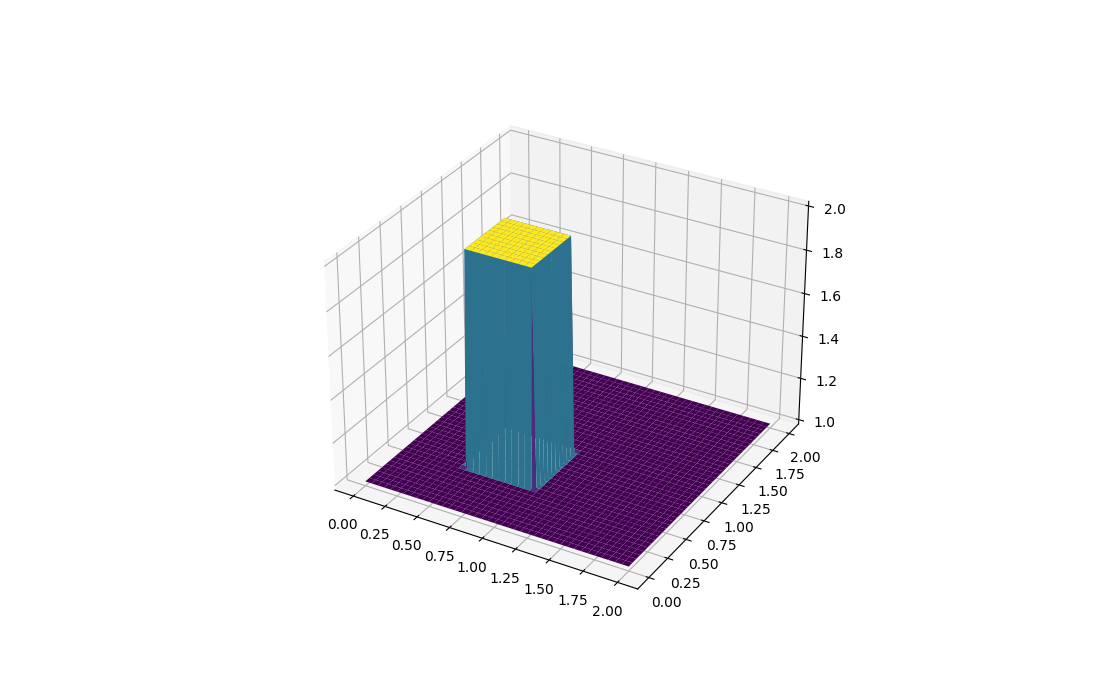
\includegraphics[width=20em]{compscieng_app45cfd3_01.png}

İki boyutta zamanı ileri saralım şimdi. Tüm $i$ ve $j$'leri işleyebilmek için
bir içiçe geçmiş döngü gerekiyor bize. Python dilinde \verb!for! kullanmak çok
optimal değildir, ama alttaki kod neler olduğunu gösterebilmek için yardımcı
olacaktır.


\begin{minted}[fontsize=\footnotesize]{python}
u = np.ones((ny, nx))
u[int(.5 / dy):int(1 / dy + 1), int(.5 / dx):int(1 / dx + 1)] = 2

for n in range(nt + 1): 
    un = u.copy()
    row, col = u.shape
    for j in range(1, row):
        for i in range(1, col):
            tmp1 = (c * dt / dx * (un[j, i] - un[j, i - 1]))
            tmp2 = (c * dt / dy * (un[j, i] - un[j - 1, i]))
            u[j, i] = (un[j, i] - tmp1 - tmp2)
            u[0, :] = 1
            u[-1, :] = 1
            u[:, 0] = 1
            u[:, -1] = 1

fig = plt.figure(figsize=(11, 7), dpi=100)
ax = fig.gca(projection='3d')
surf2 = ax.plot_surface(X, Y, u[:], cmap=cm.viridis)
plt.savefig('compscieng_app45cfd3_02.png')
\end{minted}

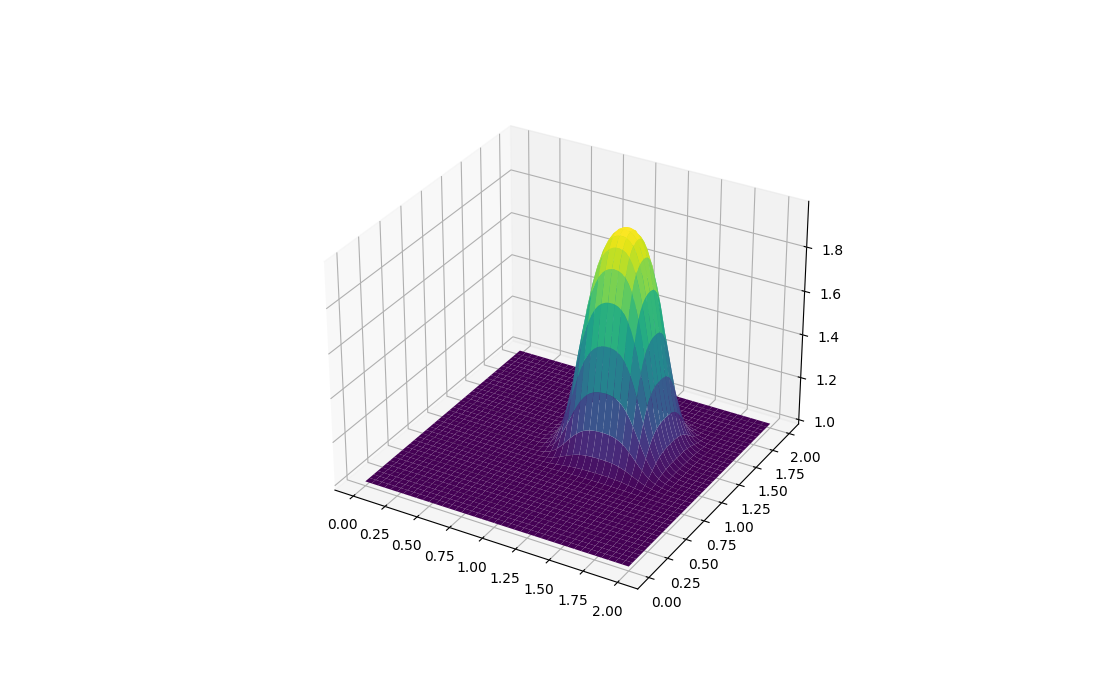
\includegraphics[width=20em]{compscieng_app45cfd3_02.png}






Kaynaklar

[1] Barba, {\em 12 steps to Navier–Stokes, Ders 1},
    \url{https://nbviewer.jupyter.org/github/barbagroup/CFDPython/blob/master/lessons/01_Step_1.ipynb}

\end{document}
